\section{Policy Enforcement}
\label{section:mechanism}

We now present the design of our policy enforcement mechanism. Although the
core of our mechanism that relies on remote memory operations is platform
agnostic, we describe it in the context of the ARM TrustZone. We leverage the
TrustZone's features to isolate the enforcement mechanism and to bootstrap its
security features. We present alternative designs in
\sectref{section:discussion:alternatives}.

\subsection{Background on ARM TrustZone}
\label{section:mechanism:armback}

The TrustZone is a set of security enhancements to chipsets based on the ARM
architecture. These enhancements cover the processor, memory and peripherals.
On TrustZone, the processor can execute instructions in one of two security
modes at any given time, a \textit{normal world} and a \textit{secure world}. A
third, \textit{monitor mode} facilitates switching between the normal and the
secure worlds.  The secure and normal worlds have their own address spaces and
different privileges.  The processor can switch from the normal world to the
secure world via an instruction called the secure monitor call (\texttt{smc}).
When an \texttt{smc} instruction is invoked from the normal world, the
processor performs a context switch to the secure world (via the monitor mode)
and freezes the execution of the normal world.

TrustZone can partition memory into two portions, with one portion being
exclusively reserved for the secure world. It also allows individual
peripherals to be assigned to the secure world.  For these peripherals,
hardware interrupts are directly routed to and handled by the secure world.
While the normal world cannot access peripherals or memory assigned to the
secure world, the secure world enjoys unrestricted access to all memory and
peripherals on the device. It can therefore access the code and data 
of the normal world. The secure world can run execute arbitrary software,
ranging from simple applications to an entire operating system.
%
% NOT the CPU state. Registers are "banked", and only monitor mode can view
% them all.

A device running ARM TrustZone boots up in the secure world. After the secure
world has initialized, it switches to the normal world and boots the operating
system there. Most TrustZone-enabled devices are configured to execute a
\textit{secure boot} sequence that incorporates cryptographic checks into the
secure world boot process~\cite{armtz}. For example, the device vendor could
sign the code with its private key, and the vendor's code in the boot ROM would
verify this signature using the vendor's public key. These checks ensure that
the integrity of the boot-time code in the secure world has not been
compromised, \eg~by reflashing the image on persistent storage. Most vendors
lock down the secure world via secure boot, thereby ensuring that it cannot be
modified by end-users. This feature allows hosts to trust software executing in
the secure world and treat it as part of the TCB. In the rest of this paper, we
will assume that our guest devices use the secure boot process.

\subsection{Overall Design}
\label{section:mechanism:overall}

\begin{figure}[t!]
\centering
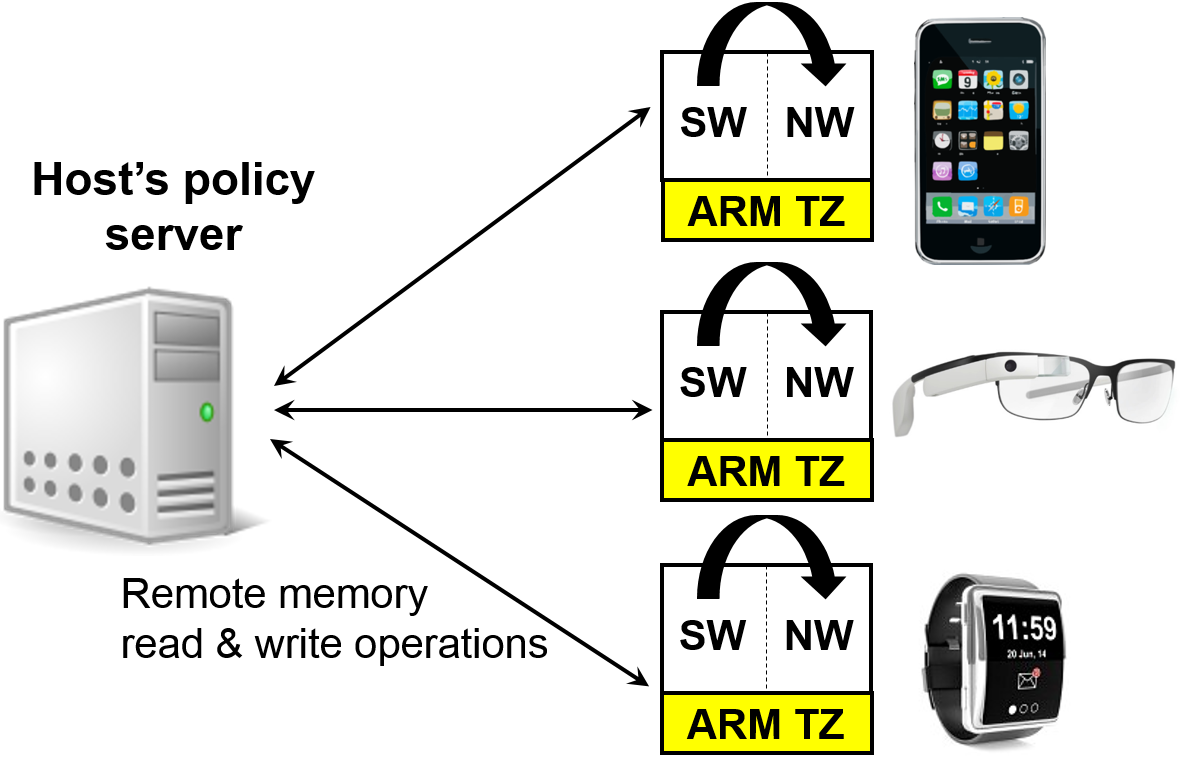
\includegraphics[keepaspectratio=true,width=0.47\textwidth]{figures/host-guest.png}
\mycaption{Overall setup showing communication between the host and guest
devices. Guest devices are equipped with ARM TrustZone and execute components
of the policy enforcement mechanism (see \figref{figure:overall}).  Abstractly,
the goal is to establish a communication channel between the host's policy
server and the enforcement mechanism running in the secure world (SW) of the
guest devices. The host leverages the secure world to remotely inspect and
modify the normal world's (NW) memory.}
{\label{figure:hostguest}}
\end{figure}

\figref{figure:hostguest} shows the overall setup of our framework. The host
runs a policy server that communicates with guest devices in its restricted
space. The normal world of each guest executes the end-user's work environment,
and can run a full-fledged mobile operating system---in our prototype the
normal world executes Android. Because this code is under the control of the
end-user, the normal world is untrusted. The secure world of the guest runs a
TCB that accepts and processes the operations remotely-initiated by the host to
inspect the guest device and regulate the use of its peripherals. 

For this setup to work, we need a communication channel that allows the host to
securely relay its requests to the guest and obtain the guest's responses. In
particular, the channel must not allow an attacker, such as the untrusted code
executing in the normal world, to tamper with messages transmitted on it.

One way to set up such a channel is to configure the secure world to directly
communicate with the host. In this case, the secure world would exclusively
control a communications peripheral, say WiFi, and establish a connection with
the host without involving the normal world. Thus, the code necessary to
support this peripheral must also execute within the secure world and be part
of the TCB. With WiFi, for instance, this would mean that several thousand
lines from the networking stack would need to execute within the TCB.

In our work, we chose an alternative approach that minimizes the functionality
implemented in the TCB. In this approach, the normal world mediates the
communication channel between the secure world and the host, and is assigned
all the peripherals on the device. Because the normal world is untrusted, the
secure world and the host include cryptographic checksums with each message
transmitted on the channel, and sanity-check the messages before processing
them. The secure world itself executes a TCB that performs just three key
operations, and the bare-minimum code needed to support these operations:
%
\begin{mylist}
%
\item~Mutual authentication (\sectref{section:mechanism:auth}), 
%
\item~Support for remote memory operations (\sectref{section:mechanism:rmo}),
%
\item~Support for verification tokens (\sectref{section:mechanism:tokens}). 
%
\end{mylist}

\begin{figure}[t!]
\centering
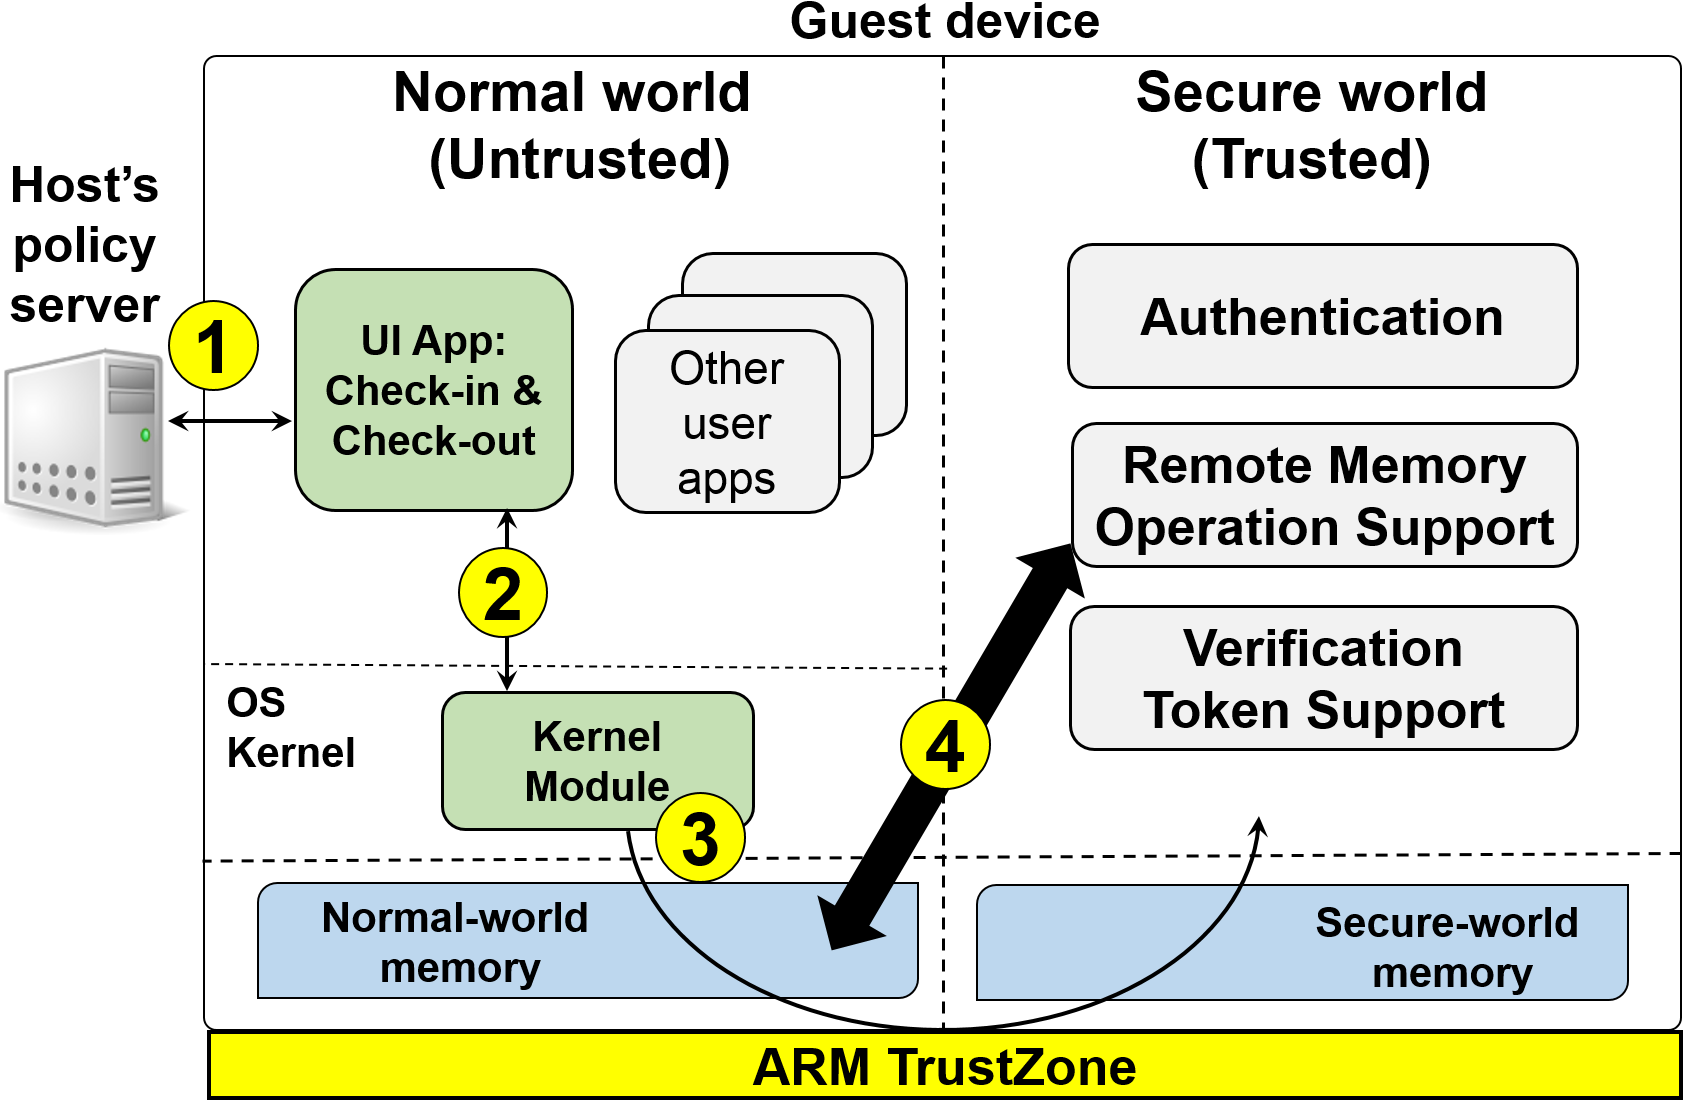
\includegraphics[keepaspectratio=true,width=0.47\textwidth]{figures/overall-design.png}
\mycaption{Guest device setup showing components of the policy enforcement
mechanism. (1)~The host communicates with the UI app on the guest and sends
requests to perform remote memory operations. (2)~The UI app forwards this
request to the supporting kernel module. (3)~The kernel module invokes the
secure world by performing a world switch. (4)~The secure world performs the
requested memory operations on the normal world memory on behalf of the host.
The components in the normal world, \ie~the UI app and the kernel module are
untrusted. The TCB consists of only the components that execute in the secure
world.}{\label{figure:overall}}
\end{figure}

Guest devices are therefore set up as shown in \figref{figure:overall}.  Within
the normal world, the end-user interacts with the host as well as with the
secure world via a user-level app (called the UI app).  This app serves as the
end-user's interface to the host, allowing him to perform operations such as
check-in and check-out of the device. The app interacts with the components in
the secure world via a kernel module. The host sends requests to perform remote
memory operations on the guest device to the app, which forwards this request
to the kernel module, which invokes \texttt{smc} to world switch into secure
world. The components of the secure world then perform the request and
communicate any return values to the host via the UI app. 

We do not place any restrictions on how the host communicates with the guest.
Thus, the host's policy server could be hosted on the cloud and communicate
with the guest device over WiFi or 3G. Alternatively, the host could install
physical scanners at a kiosk or on the entryway to the restricted space.  The
guest devices would use Bluetooth, NFC, or their USB interface to pair with the
scanner and use it to communicate with the host's policy server.

One of the key features of our approach is that the core mechanisms that run
on the TCB in the guest device are \textit{platform-agnostic} and
\textit{policy-agnostic}.  Rather, they present a narrow read/write interface
that hosts can suitably use to enforce policy. All the complex tasks of device
analysis and deciding policy are shifted to the host. Thus, in principle, we
can use the same TCB mechanisms on guest devices that run Android, iOS and
Windows. Hosts would have separate modules to analyze and control each kind of
guest platform.

\subsection{Authentication}
\label{section:mechanism:auth}
\newcommand{\ks}{$k_s$}
\newcommand{\pub}[1]{\textsf{Pub#1}}
\newcommand{\prv}[1]{\textsf{Prv#1}}
\newcommand{\enc}[2]{\textsf{Enc}$_{#1}$(#2)}
\newcommand{\cert}[1]{\textsf{Cert}(#1)}

Before accepting any remote memory requests, the guest and the host mutually
authenticate each other. We assume that both the host and the guest device have
public/private key pairs with digital certificates issued by a certifying
authority. The guest device stores its private key \prv{G} in its secure world,
thereby protecting it from the untrusted normal world. 

\begin{figure}[t!]
\footnotesize
\centering
\begin{tabular}{|rll|}
\hline
\multicolumn{3}{|l|}{Let host's public/private keypair be \pub{H},~\prv{H}.}\\
\multicolumn{3}{|l|}{Let guest's public/private keypair be \pub{G},~\prv{G}.}\\
1. & \textbf{Guest} $\rightarrow$ \textbf{Host}:
   & \pub{G}, \cert{\pub{G}}\\
%
2. & \textbf{Host} $\rightarrow$ \textbf{Guest}:
   & \pub{H}, \cert{\pub{H}}\\
%
3. & \multicolumn{2}{p{0.42\textwidth}|}{Guest and host verify
       \cert{\pub{H}} and \cert{\pub{G}}}\\
%
4. & \textbf{Host} $\rightarrow$ \textbf{Guest}:
   & $M$, \enc{\prv{H}}{$M$} (\ie~host signs $M$),\\
%
   & \multicolumn{2}{p{0.42\textwidth}|}{where $M$ is 
	      \enc{\pub{G}}{\ks, timestamp}}\\
%
5. & \multicolumn{2}{p{0.42\textwidth}|}{Guest verifies host's digital 
        signature, decrypts M to obtain \ks, and checks timestamp}\\
%
\hline
\end{tabular}
\mycaption{Mutual authentication and establishment of session key \ks.}
{\label{figure:authentication}}
\end{figure}

Authentication proceeds in a manner similar to TLS handshakes
(\figref{figure:authentication}). The host and the guest exchange public keys
and validate the certificates of these keys with the issuing authority. The
host then computes a session key \ks, which is then transmitted to the client
over an secure channel. Again, this resembles session key establishment in TLS.
The major difference is that \ks\ is only used to protect the integrity of
messages transmitted between the guest and the host and not its
confidentiality. The key \ks\ is stored in secure world memory, and is
therefore invisible to the normal world. If the guest is rebooted, \ks\ is
erased from memory.


\subsection{Remote Memory Operations}
\label{section:mechanism:rmo}

\myparagraph{Remote Reads} 
%
The host inspects and modifies the guest device's configuration via remote
memory operations. During check-in the host typically requests the guest to
send raw memory pages from the normal world for analysis.  The UI app receives
this request and performs a world switch to complete the request.  The world
switch suspends the UI app and transfers control to the secure world.  Each
request is a set of virtual memory addresses of pages that must be sent to the
host.   The host also includes a message-authentication code (a SHA1-based HMAC
in our case) with the request. The HMAC is over the body of the request using
the key \ks\ negotiated during the authentication phase.

The secure world checks the integrity of the request using the HMAC. This step
is necessary to ensure that the request was not maliciously modified by the
untrusted components in the normal world. The secure world then translates each
virtual page address in the request to a physical page address by consulting
the page table in the normal world kernel. In this case, the page table will
correspond to the suspended context in the normal world, \ie~that of the UI
app, into which the running kernel is also mapped.  It then creates a
local copy of the contents of this physical page from the normal world, and
computes an HMAC over the page (again using \ks). The page and its HMAC are
then copied to a buffer in the normal world, from where they can be transmitted
to the host by the UI app.  The host checks the HMAC and uses the page for
analysis. This process is iterative, with the host requesting more pages from
the guest based upon the results of the analysis.

Note that in our case, both the host and the secure world are isolated from the
normal world, which is untrusted. We only rely on the normal world kernel to
facilitate communication between the host and the secure world. Moreover, both
the host and the secure world check the integrity of messages communicated over
this channel, thereby preventing any attempts by the normal world kernel to
maliciously modify these messages.  The normal world may drop messages and
cause a denial-of-service attack; however, such attacks are outside our threat
model (see \sectref{section:threat}). The host can therefore reliably obtain
the memory pages of the normal world to enable the kinds of analyses described
in \sectref{section:policy:analysis}. Although the communication between the
host and the secure world is integrity-protected using HMACs, the communication
is not confidential, and is therefore not encrypted. Thus, a malicious normal
world kernel can potentially snoop on the requests from the host to fetch pages
and attempt to remove the source of infection to avoid being detected. However,
this would also have the desirable side-effect of cleaning the guest device at
check-in.

\myparagraph{Remote Writes}
%
The host reconfigures the guest by modifying the running state of the normal
world kernel via remote write requests. Each write request is a set of triples
$\langle$\textit{vaddr}$_i$,~\textit{val}$_i$,~\textit{old-val}$_i$$\rangle$
together with an HMAC of this request. The normal world conveys this request to
the secure world, which verifies the integrity of the message using its HMAC.
For each virtual address \textit{vaddr}$_i$ (which refers to a memory location
in the virtual address space of the UI app) in the request, the secure world
ensures that the current value at the address matches \textit{old-val}$_i$.  If
all the values match, then the secure world replaces their values with
\textit{val}$_i$. 

Note that because the normal world is frozen during the course of this
operation, the entire update is atomic with respect to the normal world. When
a remote write operation succeeds, the secure world computes and returns a
verification token to the host. If not, it returns an error code denoting a
failure.

A remote write request can fail if the value stored at the virtual address
\textit{vaddr}$_i$ does not match the value \textit{old-val}$_i$.  This problem
arises in our design because the host's remote read and write operations do not
happen as an atomic unit. The host remotely reads pages copied from the normal
world's memory, analyzes them and creates remote write request using this
analysis. During this time, the normal world kernel continues to execute, and
may either have updated the value at the virtual address \textit{vaddr}$_i$.

If a remote write operation fails, the host repeats the operation until it
succeeds. That is, it refetches pages from the guest, analyzes them, and
creates a fresh write request. In theory, it is possible that the host's write
requests will fail \textit{ad infinitum}. However, for the setting that we
consider, write operation failures are rare in practice. This is because our
write operations modify the addresses of peripheral device driver hooks.
Operating systems typically do not change the values of device driver hooks
after they have been initialized at system boot. 

In theory, a remote write request can also fail if the virtual address
\textit{vaddr}$_i$ referenced in the request is not mapped to a physical page
in memory, \ie~if the corresponding page has been swapped out to persistent
storage. In practice, however, we restrict remote writes to kernel data pages
that are resident in physical memory, as is the case with device drivers and
pages that store data structures of peripherals. Therefore, we do not observe
failures due to a failure to resolve \textit{vaddr}$_i$s.

It is possible to completely avoid such problems by design if we complete both
the read and write operations in a single world switch. During this time, the
normal world remains frozen and cannot change the view of memory exported to
the host.  The read and write operations will therefore happen as an atomic
unit from the normal world's perspective. However, in this case, the secure
world must have the ability to directly communicate with the host. As already
discussed in \sectref{section:mechanism:overall}, we decided against this
design because it has the unfortunate consequence of bloating the size of the
TCB.  Thus, we make the practical design tradeoff of minimizing the
functionality of the TCB while allowing the rare remote write failure to
happen.

\subsection{Verification Tokens}
\label{section:mechanism:tokens}

The host receives a verification token from the secure world upon successful
completion of a remote write operation. A verification token \textsf{VTok}[$r$]
is the value: 
%
$$ \textsf{VTok}[r] =
r||\textit{MemState}||\textsf{HMAC}_{k_s}[r||\textit{MemState}] $$ 
%
where \textit{MemState} is
$\langle\textit{vaddr}_1,~\textit{val}_1\rangle||\ldots||\langle\textit{vaddr}_n,~\textit{val}_n\rangle$,
the set of \textit{vaddr}$_i$ modified by the remote write, and the new values
\textit{val}$_i$ at these locations. The token \textsf{VTok}[$r$] is
parameterized by a random nonce $r$. This nonce can either be provided by the
host together with the remote write request, or can be generated by the secure
world. 

Verification tokens allow the host to determine whether the guest attempted to
revert the configuration changes made by the remote write, either maliciously
or by turning off the guest device. To do so, the host obtains a verification
token \textsf{VTok}[$r_{\textit{checkin}}$] upon completion of checkin, and
stores this token for validation. During checkout, the host requests a
validation token \textsf{VTok}[$r_\textit{checkout}$] from the guest over the
same virtual memory addresses. The secure world accesses each of these memory
addresses and computes the verification token with $r_\textit{checkout}$ as the
nonce. The host can compare the verification tokens
\textsf{VTok}[$r_{\textit{checkin}}$] and
\textsf{VTok}[$r_{\textit{checkout}}$] to determine whether there were any
changes to the values stored at these memory addresses. 

Assuming a good source of randomness, the nonces $r_\textit{checkin}$ and
$r_\textit{checkout}$ ensure the freshness of the tokens
\textsf{VTok}[$r_{\textit{checkin}}$] and
\textsf{VTok}[$r_{\textit{checkout}}$].  The use of the  \ks\ to compute the
HMAC in the verification token ensures that the token is only valid for the
duration of the session, \ie~until check-out or until the device is powered
off, whichever comes earlier. Because \ks\ is only stored in secure world
memory, it is ephemeral and unreadable to the normal world. This ensures that
any attempts, either malicious or benign, to undo the configuration changes
induced by the remote writes at check-in will be detected by the host.

% \subsection{Security Analysis}
% What if kernel module is loaded dynamically? We disable that.

